\documentclass[a4paper,11pt]{article}

\usepackage[utf8]{inputenc}
\usepackage[T1]{fontenc}
\usepackage[english]{babel}
\usepackage{graphicx}
\usepackage{amsmath,amssymb,amsthm,amsopn}
\usepackage{mathrsfs}
\usepackage{graphicx}
\usepackage{array}
\usepackage{makecell}


\usepackage{hyperref}
\hypersetup{
    colorlinks=true,
    linkcolor=blue,
    citecolor=red,
}

%\usepackage[top=1cm,bottom=1cm]{geometry}
%\usepackage{listings}
%\usepackage{xcolor}

\usepackage{tikz}

% Tikz style

\tikzset{round/.style={circle, draw=black, very thick, scale = 0.7}}
\tikzset{arrow/.style={->, >=latex}}
\tikzset{dashed-arrow/.style={->, >=latex, dashed}}

\newtheoremstyle{break}%
{}{}%
{\itshape}{}%
{\bfseries}{}%  % Note that final punctuation is omitted.
{\newline}{}

\newtheoremstyle{sc}%
{}{}%
{}{}%
{\scshape}{}%  % Note that final punctuation is omitted.
{\newline}{}

\theoremstyle{break}
\newtheorem{thm}{Theorem}[section]
\newtheorem{lm}[thm]{Lemma}
\newtheorem{prop}[thm]{Proposition}
\newtheorem{cor}[thm]{Corollary}

\theoremstyle{sc}
\newtheorem{exo}{Exercice}

\theoremstyle{definition}
\newtheorem{defi}[thm]{Definition}
\newtheorem{ex}[thm]{Example}

\theoremstyle{remark}
\newtheorem{rem}[thm]{Remark}

% Math Operators

\DeclareMathOperator{\Card}{Card}
\DeclareMathOperator{\Gal}{Gal}
\DeclareMathOperator{\Id}{Id}
\DeclareMathOperator{\Img}{Im}
\DeclareMathOperator{\Ker}{Ker}
\DeclareMathOperator{\Minpoly}{Minpoly}
\DeclareMathOperator{\Mod}{mod}
\DeclareMathOperator{\Ord}{Ord}
\DeclareMathOperator{\ppcm}{ppcm}
\DeclareMathOperator{\Tr}{Tr}
\DeclareMathOperator{\Vect}{Vect}

% Shortcuts

\newcommand{\dE}{\partial(E)}
\newcommand{\dF}{\partial(F)}
\newcommand{\dG}{\partial(G)}
\newcommand{\diff}{\mathop{}\!\mathrm{d}}
\newcommand{\eg}{\emph{e.g. }}
\newcommand{\emb}{\hookrightarrow}
\newcommand{\embed}[2]{\phi_{#1\hookrightarrow#2}}
\newcommand{\ent}[2]{[\![#1,#2]\!]}
\newcommand{\ie}{\emph{i.e. }}
\newcommand{\ps}[2]{\left\langle#1,#2\right\rangle}





% opening
\title{Notes on compatible composita}
\author{}



\begin{document}

\maketitle

%\begin{abstract}

%\end{abstract}

%\tableofcontents

%\clearpage

In this document, we investigate compatibility questions in the case of the
compositum of two finite fields $\mathbb{F}_{p^m}$ and $\mathbb{F}_{p^n}$, where
the integers $m$ and $n$ are coprime. In that case, the compositum is
$\mathbb{F}_{p^{mn}}$. We denote by $\zeta_m$ (resp. $\zeta_n$) a primitive $m$-th 
root of unity (resp. $n$-th). We set $\alpha_m$ a solution of Hilbert 90 in
$\mathbb{F}_{p^m}\otimes\mathbb{F}_{p}(\zeta_m)$ for the root $1\otimes\zeta_m$,
and we similarly set $\alpha_n$. Let now $u, v$ be integers such that
\[
  un+vm = 1.
\]
We now set
\[
  \zeta=\zeta_m^u\zeta_n^v
\]
and 
\[
  \alpha=\alpha_m^u\alpha_n^v,
\]
such that $\zeta$ is a primitive $mn$-th root of unity, $\zeta^m=\zeta_n$,
$\zeta^n=\zeta_m$ and $\alpha$ is a
solution of Hilbert 90 in $\mathbb{F}_{p^{mn}}\otimes\mathbb{F}_{p}(\zeta)$ for
the root $1\otimes\zeta$. We also have that
\[
  (\sigma\otimes\Id)(\alpha^n) = (1\otimes\zeta_m)\alpha^n
\]
and
\[
  (\sigma\otimes\Id)(\alpha^m) = (1\otimes\zeta_n)\alpha^m
\]
but not necessarily $\alpha^n=\alpha_m$ and $\alpha^m=\alpha_n$. In fact we have 
\begin{align*}
  \alpha^n &= \alpha_m^{un}\alpha_n^{vn} \\
  &= \alpha_m^{1-vm}a_n^v \\
  &= \cfrac{a_n^v}{a_m^v}\alpha_m
\end{align*}
where $a_m=\alpha_m^m\in\mathbb{F}_p(\zeta_m)$ and $a_n =
\alpha_n^n\in\mathbb{F}_p(\zeta_n)$. We also get
\[
  \alpha^m = \cfrac{a_m^u}{a_n^u}\alpha_n
\]
in the same way.
\section{Example with $p=7$, $m=2$, $n=3$}
Let us start with an example where we do not have to worry about tensor
products, because all the needed roots are in the prime field. We take $p=7$,
$m=2$ and $n=3$. Since $p-1=6$ is divisible by both $2$ and $3$, we have
primitive $2$-th and $3$-th roots of unity in $\mathbb{F}_7$. We investigate the
possible embeddings $\mathbb{F}_{7^2}\emb\mathbb{F}_{7^6}$ and
$\mathbb{F}_{7^3}\emb\mathbb{F}_{7^6}$, as shown in Figure~\ref{fig:p7}.
\begin{figure}
  \centering
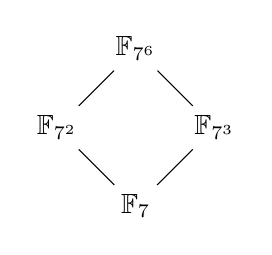
\begin{tikzpicture}
  \node (1) at (0,0) {$\mathbb{F}_{7}$};
  \node (2) at (-1,1) {$\mathbb{F}_{7^2}$};
  \node (3) at (1,1) {$\mathbb{F}_{7^3}$};
  \node (6) at (0,2) {$\mathbb{F}_{7^6}$};

  \draw (1) -- (2);
  \draw (1) -- (3);
  \draw (2) -- (6);
  \draw (3) -- (6);
\end{tikzpicture}
\phantom{and}
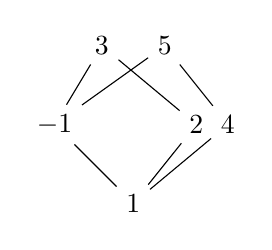
\begin{tikzpicture}
  \node (1) at (0,0) {$1$};
  \node (-1) at (-1,1) {$-1$};
  \node (2) at (0.8,1) {$2$};
  \node (4) at (1.2,1) {$4$};
  \node (3) at (-0.4,2) {$3$};
  \node (5) at (0.4,2) {$5$};

  \draw (1) -- (2);
  \draw (1) -- (-1);
  \draw (1) -- (4);
  \draw (-1) -- (3);
  \draw (-1) -- (5);
  \draw (2) -- (3);
  \draw (4) -- (5);
\end{tikzpicture}
  \caption{Compositum with $p=7$, $m=2$, $n=3$, and the associated roots.}
  \label{fig:p7}
\end{figure}
In the same picture, we see that we have one primitive $2$-th root of unity that
is $-1$, two primitive $3-th$ roots of unity that are $2$ and $4$ and two
primitive $6$-th roots of unity that are $3$ and $5$. We have the compatibility
relations $3^3=5^3=-1$, $3^2=2$ and $5^2=4$.

We define 
\[
  \mathbb{F}_{7^2}\cong \mathbb{F}_7[y]/(y^2-3)\cong \mathbb{F}_7(u),
\]
\[
  \mathbb{F}_{7^3}\cong \mathbb{F}_7[x]/(x^3-2)\cong \mathbb{F}_7(t),
\]
and
\[
  \mathbb{F}_{7^6}\cong \mathbb{F}_7[z]/(z^6-5)\cong \mathbb{F}_7(w).
\]
We embed $\mathbb{F}_{7^2}$ in $\mathbb{F}_{7^6}$ by sending $u$ to $w^3$ and we
embed $\mathbb{F}_{7^3}$ in $\mathbb{F}_{7^6}$ by sending $t$ to $3w^4$.

\end{document}
